%!TEX program = xelatex

\documentclass[cn,hazy,green,11pt,device=normal,chinesefont=founder]{elegantnote}

\newcommand{\frontface}
{
\clearpage % 加这个命令后, 目录中的页码才显示正确
\phantomsection % 加这个命令后, 目录中的超链接才指向正确的页码
\section*{前言} %开始一段不带编号的章
\addcontentsline{toc}{section}{前言} %使目录中以章级别显示“致谢”
}

\title{\textcolor{black}{\Huge{量子场论笔记(Peskin \& Schroeder)}}}

\author{\textcolor{black}{Toki \& Starry}}
\institute{}

% \version{0.01}
\date{\today}

\usepackage{array}
\usepackage{graphicx}

\begin{document}

\maketitle

\mbox{}

\centerline{
  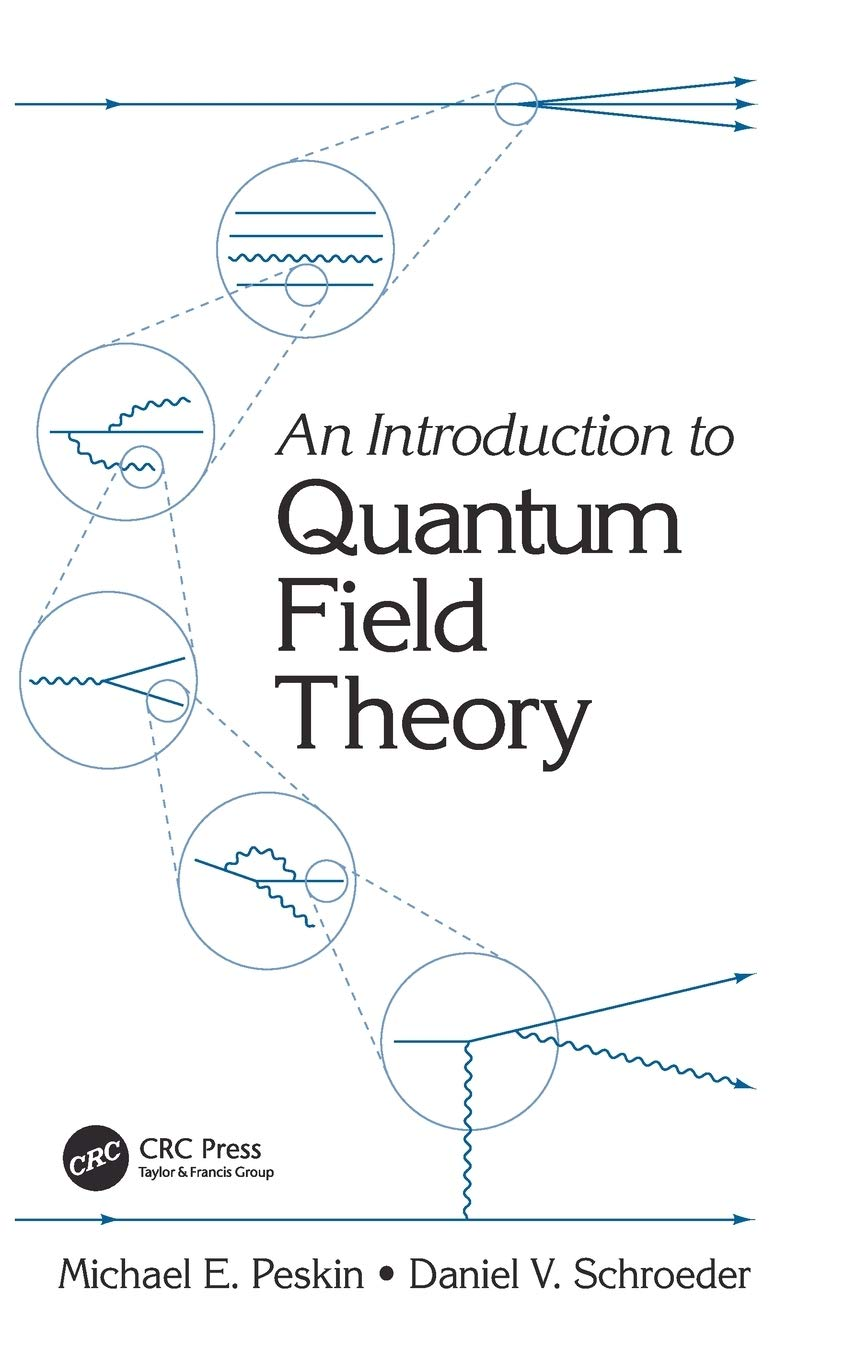
\includegraphics[width=0.72\textwidth]{peskin-front.jpg}
}

\tableofcontents

\clearpage

\frontface

本文为基于\textit{An Introduction to Quantum Field Theory} - \textit{Peskin \& Schroeder}的量子场论笔记. 

本文主要对此书正文部分一些复杂的计算和难以理解的段落作了注释, 同时根据研究生课程内容对部分较为简略的段落添加了补充说明. 由于计算比较困难, 并且许多概念及物理图像需要仔细思考后才能理解, 故本篇笔记将以中文呈现. 若后有闲暇, 将转译为英文. 

如发现任何错误或遗漏, 或希望与我讨论书中的内容, 欢迎通过\href{mailto:toshiko.h19@gmail.com}{邮件}联系. 

邮箱: \texttt{toshiko.h19@gmail.com}

本文大量参考了\href{http://gamebm.shoutwiki.com/wiki/Lecture_Notes_of_An_Introduction_to_Quantum_Field_Theory_by_M._Peskin_and_D._Schroeder}{这篇笔记}. 谢谢你, 陌生人. 

\clearpage

\section{Invitation: Pair Production in \texorpdfstring{$e^+e^-$} Annihilation}

介绍性的章节. 

可能有一些有意思的内容, 暂时跳过. 

\clearpage

\section{The Klein-Gordon Field}

\subsection{The Necessity of the Field Viewpoint}

这里提到需要将场量子化的一个原因是:  由于爱因斯坦关系$E = mc^2$的存在, 任何相对论性过程中都有可能出现正负粒子对, 所以用只对单个粒子进行了量子化的理论去解释是不够的. 而对于能量较低的情况, 我们可以考虑一个存在时间极短的态, 此时由于不确定性原理$\Delta E \cdot \Delta t = \hbar /2$的存在, 会产生很多“虚粒子”, 所以\textit{量子场论}, 或着说可以处理数目不定的自由度的相对论性量子理论是必要的. 

同时还有一个原因是关于因果性的. 下面的计算就是经典理论中关于传播振幅$U(t)$的计算, 结果表明它们违背了因果律. 

\begin{note}
  \mbox{}
  \begin{enumerate}
    \item 关于场的简单理解

      在三维空间中, 有$n$个自由度的系统共有$a=3n$个广义坐标, 每个广义坐标可以写为$q_a$. 而当我们考虑无限自由度时, $a$变为连续参数, $q_a$变为函数$q(a)$, 于是我们便得到了“场”. (这是非常粗略的描述, 具体如何从离散变量过渡到场可以参考\textit{Goldstein}第13章) 
  
      或者可以把场理解为某种实体在时空中的分布, 它是时空坐标$x^\mu$的函数, 是一个基础的力学量. 

    \mbox{}

    \item 常用的场
    \begin{itemize}
      \item $\phi(x)$: 标量场(比如希格斯场)
      \item $A_\mu(x)$: 矢量场(电磁场)
      \item $\psi(x)$: 旋量场
    \end{itemize}
  \end{enumerate}
\end{note}

\subsubsection{P.14 - Eq-1}

当$E = \mathbf{p}^2/2m$时,
\begin{equation}
  \displaybreak
  \begin{aligned}
  U(t) &= \langle \mathbf{x}|e^{-i(\mathbf{p}^2/2m)t}|\mathbf{x}_0\rangle \\ 
       &= \int d^3p \langle \mathbf{x}| e^{-i(\mathbf{p}^2/2m)t} |\mathbf{p}\rangle \langle \mathbf{p}| \mathbf{x}_0 \rangle \\ 
       &= \int d^3p \ e^{-i(\mathbf{p}^2/2m)t} \langle \mathbf{x}|\mathbf{p}\rangle \langle \mathbf{p}| \mathbf{x}_0\rangle \\ 
       &= \int d^3p \ e^{-i(\mathbf{p}^2/2m)t} \biggl(\frac{1}{2\pi}\biggr)^\frac{3}{2} e^{i\mathbf{p}\cdot\mathbf{x}} \biggl(\frac{1}{2\pi}\biggr)^\frac{3}{2} e^{-i\mathbf{p}\cdot\mathbf{x}_0} \\ 
       &= \frac{1}{(2\pi)^3} \int d^3p \ e^{-i(\mathbf{p}^2/2m)t} e^{i\mathbf{p}\cdot(\mathbf{x}-\mathbf{x}_0)} \\
       &= \biggl(\frac{m}{2\pi it}\biggr)^\frac{3}{2} e^{im(\mathbf{x}-\mathbf{x}_0)^2/2t} . 
  \end{aligned}
\end{equation}
  
最后一步直接使用高斯积分公式. 

\begin{note}
一维高斯积分公式
\begin{equation}
\int_{-\infty}^{\infty}dx\ e^{-cx^2}e^{\pm ibx} = \sqrt{\frac{\pi}{c}}e^{-b^2/4c}. 
\end{equation}
\end{note}

\subsubsection{P.14 - Eq-2}

当$E = \sqrt{\mathbf{p}^2+m^2}$时, 
\begin{equation}
  \begin{aligned}
  U(t) &= \mathinner{\langle \mathbf{x}|}e^{-it\sqrt{\mathbf{p}^2+m^2}}\mathinner{|\mathbf{x}_0\rangle} \\
       &= \frac{1}{(2\pi)^3} \int d^3p \ e^{-it\sqrt{\mathbf{p}^2+m^2}} e^{i\mathbf{p}\cdot(\mathbf{x}-\mathbf{x}_0)} \\ 
       &= \frac{1}{(2\pi)^3} \int p^2\sin\theta dp d\theta d\varphi \ e^{-it\sqrt{p^2+m^2}} e^{ip|\mathbf{x}-\mathbf{x}_0|\cos\theta} \\ 
       &= \frac{1}{(2\pi)^2} \int_0^\infty p^2 dp \ e^{-it\sqrt{p^2+m^2}} \int_0^\pi d\theta \sin\theta \ e^{ip|\mathbf{x}-\mathbf{x}_0|\cos\theta} \\
       &= -\frac{i}{(2\pi)^2|\mathbf{x}-\mathbf{x}_0|} \int_0^\infty dp \ p\ e^{-it\sqrt{p^2+m^2}} \int_0^\pi d(ip|\mathbf{x}-\mathbf{x}_0|\cos\theta) \ e^{ip|\mathbf{x}-\mathbf{x}_0|\cos\theta} \\
       &= -\frac{i}{(2\pi)^2|\mathbf{x}-\mathbf{x}_0|} \int_0^\infty dp \ p\ e^{-it\sqrt{p^2+m^2}} (e^{-ip|\mathbf{x}-\mathbf{x}_0|}-e^{ip|\mathbf{x}-\mathbf{x}_0|}) \\
       &= \frac{1}{2\pi^2|\mathbf{x}-\mathbf{x}_0|} \int_0^\infty dp \ p\ \sin(p|\mathbf{x}-\mathbf{x}_0|) e^{-it\sqrt{p^2+m^2}}. 
  \end{aligned}
\end{equation}

第三行中, 我们把向量$(\mathbf{x}-\mathbf{x}_0)$的方向设为了$z$-axis的正方向. 

\subsubsection{P.15 - Figure 2.1}

两个事件之间的间隔是洛伦兹标量, 即
\begin{equation}
  (x-x_0)^2 = -s^2,
\end{equation}
因为是类空间隔, 所以有个负号. 

我们把$x_0$作为原点, 令$x'=x-x_0$, 空间分量只考虑一维($x'=(t',x')$), 则有
\begin{equation}
  x'^2-t'^2=s^2,
\end{equation}
这就是洛伦兹变换下$x'$满足的关系, 即为图中所画的双曲线. 

\subsection{Elements of Classical Field Theory}

注意这里在讨论初末状态时, 直接将时空坐标零分量$x^0$取为了定值. 实际上在不同的空间点, 初末状态的$x^0$可以取不同的值, 只需要保证边界是类空超曲面即可. 

\begin{remark}
  我的理解: 只有这样在向空间的无穷远处积分时才能到达时间上的边界. 可以画个图感受一下. 
\end{remark}

\subsubsection{P15 - (2.2) (2.3)}

这里的
\begin{equation}
  \frac{\partial \mathcal{L}}{\partial(\partial_\mu \phi)}\delta(\partial_\mu \phi),
\end{equation}
具体可以写成
\begin{equation}
  \frac{\partial \mathcal{L}}{\partial\dot\phi}\delta  \dot{\phi}+\frac{\partial \mathcal{L}}{\partial(\boldsymbol{\nabla} \phi)}\delta(\boldsymbol{\nabla} \phi),
\end{equation}
这里和下面的计算中出现的都不是四矢量的内积, 而是各分量偏微分的和的简写(可以全部展开算一遍). 于是最后的Euler-Lagrange equation也可以写为
\begin{equation}
  \frac{\partial}{\partial t}\biggl(\frac{\partial \mathcal{L}}{\partial\dot\phi}\biggr) + \boldsymbol{\nabla} \biggl(\frac{\partial \mathcal{L}}{\partial(\boldsymbol{\nabla} \phi)}\biggr) - \frac{\partial \mathcal{L}}{\partial \phi} = 0,
\end{equation}
这在利用薛定谔场的 Lagrangian 导出薛定谔方程的时候很有用. 

而关于这里的边界项$\partial_\mu \bigl(\frac{\partial \mathcal{L}}{\partial(\partial_\mu \phi)}\delta \phi \bigr)$, 注意要分别考虑时间和空间分量(书中也提到了). 

\begin{note}
  薛定谔场的Lagrangian为
  \begin{equation}
    \mathcal{L}_{Schr\ddot{o}dinger} = i\hbar\psi^\dagger\frac{\partial \psi}{\partial t} - \frac{\hbar^2}{2m}\boldsymbol{\nabla}\psi^\dagger\boldsymbol{\nabla}\psi - V(\mathbf x)\psi^\dagger\psi.
  \end{equation}
\end{note}

\subsubsection{P16 - Hamiltonian Field Theorem}

这里关于哈密顿形式的场论并没有讲完(没有导出运动方程). 导出运动方程要给出场变量和其共轭动量之间的对易/反对易关系, 再计算Heisenberg equation得到运动方程. 

\begin{note}
  Heisenberg equation
  \begin{equation}
    i\frac{\partial}{\partial t}\mathcal{O} = [\mathcal{O}, H].
  \end{equation}
\end{note}

Hamiltonian Field Theorem实际上是和Lagrangian Field Theorem不同的路径. 而为了保证它能给出正确的运动方程, 正则量子化的方法只有两种, 也就是上面提到的(等时)对易/反对易关系. 

\subsubsection{P17 - Noether's Theorem}

这里可以参考Hagen Kleinert课件中的\href{http://users.physik.fu-berlin.de/~kleinert/b6/psfiles/Chapter-7-conslaw.pdf}{解释}以及Weinberg QFT第一册中的7.3节. 

Hagen Kleinert解释了在(2.11)中用Euler-Lagrange方程的含义: 在此处我们只考虑由最小作用量原理决定的那个场分布, 因此可以用Euler-Lagrange方程简化表达式. 即在所有的场分布中, 我们仅考虑了\textit{真实}的场分布(即经典力学中粒子运动的真实轨道). 

我此前的疑惑是: 由书中(2.11)推导, 任意的全局变换($\alpha$ 为常数)都会导致Lagrangian变化一个4-divergence, 这是不是意味着任意的全局变换都是对称变换呢? 实际上, 这是因为在(2.11)中我们只考虑了\textit{真实}的场分布; 而根据Weinberg的说法, 对于\textit{真实}的场分布, 确实任意变换都会使(2.10)成立. 但\textit{对称变换}的含义是该变换使得 (2.10)对任意场分布都成立, 而不仅仅是对\textit{真实}的场分布成立, 所以“任意的全局变换都是对称变换”肯定是错误的. 

所以关于Noether's theorem, 我的理解是这样的: 

\begin{enumerate}
  \item 若某个变换是一个对称变换, 则它会使系统的Lagrangian保持不变, 或是变化至多一个4-divergence, 即(2.10). 需要注意的是, 这个变化对于系统中所有的场分布都成立, 无论是否是满足最小作用量原理的那一个. 
  \begin{remark}
    在实际计算时, 我们应该首先检查变换是否保证了(2.10)成立(书中的前两个例子都是这么做的), 并由此得到$\mathcal{J}^{\mu}$的形式. 
  \end{remark}
  \item 对于某个具体的变换(2.9), 我们可以计算得到(2.11)式, 这代表了该变换导致的Lagrangian的变化(对所有的场分布); 而接下来, 对于真实(满足最小作用量原理)的场来说, 考虑其Lagrangian的变化时, 可用Euler-Lagrange方程去掉(2.11)式中第二项; 最后, 由于剩余的一项依旧需要满足(2.10), 所以我们令它等于前面的$\mathcal{J}^{\mu}$, 得到守恒流. 
  \begin{remark}
    这一步只是为了得到守恒流的表达式. 
  \end{remark}
\end{enumerate}

\begin{note}
  \mbox{}
  \begin{enumerate}
    \item 实际上这里的导数需要替换为李导数. 
    \item 更好的导出守恒流的方式也许是考虑局域变换, 详见Weinberg书中讲解或Hagen Kleinert课件中 8.1.2 一节. 
  \end{enumerate}
\end{note}

\subsubsection{P18 - (2.13)}
\begin{equation}
  \begin{aligned}
  \frac{dQ}{dt} &= \int \partial_0 j^0 d^3 x \\
  &= \int (\partial_\mu j^\mu - \boldsymbol{\nabla}\cdot\mathbf{j}) \ d^3 x \\
  & = - \int \boldsymbol{\nabla}\cdot\mathbf{j}\ \ d^3 x \\
  &=0.
  \end{aligned}
\end{equation}

\subsection{The Klein-Gordon Field as Harmonic Oscillators} 

\subsubsection{P20 - (2.21) \textasciitilde \ (2.28)} \label{subsubsec:KG_Field_expression}

这里有一种更好的导出标量场表达式的方法. 

首先我们把对易关系修改为\textit{等时对易关系}: 
\begin{equation}
  \bigl[\phi(t, \mathbf{x}), \pi(t, \mathbf{y})\bigr] = i\delta^{(3)}(\mathbf{x} - \mathbf{y}), 
\end{equation}
而后将$\phi(x)$表达为
\begin{equation}
  \phi(\mathbf{x}, t) = \int \frac{d^3 p}{(2\pi)^3}e^{i\mathbf{p \cdot x}}\phi(\mathbf{p}, t), 
\end{equation}
其中的$\phi(\mathbf{p}, t)$为(在上式中同时对两端做积分 $\int e^{-i\mathbf{p'\cdot x}} d^3 x$ )
\begin{equation}
  \phi(\mathbf{p}, t) = \int d^3 x\ e^{-i\mathbf{p \cdot x}}\phi(\mathbf{x}, t), 
\end{equation}
由于$\phi^\dagger = \phi$ ($\phi$为实标量场), 
\begin{equation}
  \phi^{\dagger}(\mathbf{p}, t) = \int d^3 x\ e^{i\mathbf{p \cdot x}}\phi(\mathbf{x}, t) = \phi(-\mathbf{p}, t). 
\end{equation}

接下来考虑运动方程(2.21), 写出试解: 
\begin{equation}
  \phi(\mathbf{p}, t) = a_1(\mathbf{p})e^{-i\omega_p t} + a_2(\mathbf{p})e^{i\omega_p t}, 
\end{equation}
而
\begin{equation}
  \phi^{\dagger}(\mathbf{p}, t) = a_1^{\dagger}(\mathbf{p})e^{i\omega_p t} + a_2^{\dagger}(\mathbf{p})e^{-i\omega_p t}. 
\end{equation}

而$\phi^{\dagger}(\mathbf{p}, t) = -\phi(\mathbf{p}, t)$, 则
\begin{equation}
  \left\{\begin{array}{c} a_1^{\dagger}(\mathbf{p}) = a_2(\mathbf{-p})\\ a_2^{\dagger}(\mathbf{p}) = a_1(\mathbf{-p})\end{array}\right..
\end{equation}

于是$\phi(x)$可以表示为(将$a_1(\mathbf{p})$替换为$\frac{1}{\sqrt{2\omega_\mathbf{p}}} a(\mathbf{p})$): 
\begin{equation}
  \begin{aligned}
  \phi(\mathbf{x}, t) &= \int \frac{d^3 p}{(2\pi)^3}e^{i\mathbf{p \cdot x}}\Bigl(a_1(\mathbf{p})e^{-i\omega_p t} + a_2(\mathbf{p})e^{i\omega_p t}\Bigr) \\
  &= \int \frac{d^3 p}{(2\pi)^3}\Bigl(a_1(\mathbf{p})e^{-i\omega_p t +i\mathbf{p \cdot x}} + a_1^{\dagger}(-\mathbf{p})e^{i\omega_p t+i\mathbf{p \cdot x}}\Bigr) \\
  &= \int \frac{d^3 p}{(2\pi)^3}\Bigl(a_1(\mathbf{p})e^{-i\omega_p t + i\mathbf{p \cdot x}} + a_1^{\dagger}(\mathbf{p})e^{i\omega_p t - i\mathbf{p \cdot x}}\Bigr) \\
  &= \int \frac{d^3 p}{(2\pi)^3} \frac{1}{\sqrt{2 \omega_\mathbf{p}}} \Bigl(a(\mathbf{p})e^{-ipx} + a^{\dagger}(\mathbf{p})e^{+ipx}\Bigr). 
  \end{aligned}
\end{equation}

值得注意的是, 书中把$a(\mathbf{p})$写为了$a_\mathbf{p}$, 实际上理解为函数就可以了. 熟悉了以后这样写比较方便. 

\begin{remark}[个人理解]
  量子化的步骤: 引入正则对易关系, 然后解对应的运动方程. 
  
  例如这里我们首先引入对易关系使得基础力学量$\phi(x),\pi(x)$成为了算符, 然后尝试解K-G方程. 由于量子化后的方程形式和经典情形下的相同, 我们便可以从经典解出发进行尝试. 而对于微分方程, 只要能试出正确的解并验证其完备性, 就可以将其作为通解.  
\end{remark}

\subsubsection{P21 - (2.26)下面那一段}

关于求$a_\mathbf{p}$和$a^{\dagger}_\mathbf{p}$的表达式: 将(2.25)和(2.26)系数凑合适, 加减消去其中一个后, 再同时对两端做积分$\int e^{-i\mathbf{p'\cdot x}} d^3 x$即可. 

\begin{remark}
  确实很easy, Peskin没有骗你. 
\end{remark}

\subsubsection{P22 - (2.33)}

此处计算(以及相关的许多计算)可能要用到如下的关系: 
\begin{equation}
  \begin{aligned}
  \int_{-\infty}^{+\infty}\frac{d^3 p}{(2\pi)^3}f(\mathbf p) &= \int_{+\infty}^{-\infty}\frac{d^3 (-p)}{(2\pi)^3}f(-\mathbf p) \\
  &= -\int_{+\infty}^{-\infty}\frac{d^3 p}{(2\pi)^3}f(-\mathbf p) \\
  &= \int_{-\infty}^{+\infty}\frac{d^3 p}{(2\pi)^3}f(-\mathbf p).
  \end{aligned}
\end{equation}

\subsubsection{P22 - (2.34)}

建议记这个公式: 
\begin{equation}\label{eq: delta_on_function}
  \delta(f(x)) = \sum_i \frac{\delta(x-x_i)}{|f'(x_i)|}, 
\end{equation}
其中$x_i$是$f(x)$的根. 参考 \href{https://zh.wikipedia.org/wiki/狄拉克δ函数#與函數的復合}{$\delta$函数的维基百科页面}. 

\subsubsection{P23 - (2.40)} \label{subsubsec: Invar_Delta}

我们计算另一个类似的不变积分, $\Delta(x; m)$. 

\begin{definition}[Invariant Delta-Function]
  \begin{equation}
    \Delta(x; m) = -i\int\frac{d^3 p}{(2\pi)^3} \frac{1}{2E_\mathbf{p}}(e^{-ipx} - e^{+ipx}). 
  \end{equation}
\end{definition}

$\Delta(x; m)$可写为洛伦兹不变的形式(其中$\varepsilon(x)$为符号函数): 
\begin{equation}
  \Delta(x; m) = -i\int \frac{d^4 p}{(2\pi)^4}(2\pi)\varepsilon(p_0) \delta(p^2 - m^2)e^{-ipx}, 
\end{equation}

\begin{proof}
  \begin{equation}
    \begin{aligned}
      r. h. s. &= -\frac{i}{(2\pi)^3}\int d^3 p \biggl\{ \int_{0}^{\infty}dp^0\delta\Bigl((p^0)^2 - E_\mathbf{p}^2\Bigr)e^{-ipx} - \int_{-\infty}^{0}dp^0\delta\Bigl((p^0)^2 - E_\mathbf{p}^2\Bigr)e^{-ipx} \biggr\} \\
               &= -\frac{i}{(2\pi)^3}\int d^3 p \biggl\{ \int_{0}^{\infty}dp^0\frac{1}{2E_\mathbf{p}}\Bigl[\delta(p^0 - E_\mathbf{p}) + \delta(p^0 + E_\mathbf{p}) \Bigr]e^{-ipx} \\
               &\qquad \qquad \qquad \quad - 
               \int_{-\infty}^{0}dp^0\frac{1}{2E_\mathbf{p}}\Bigl[\delta(p^0 - E_\mathbf{p}) + \delta(p^0 + E_\mathbf{p}) \Bigr]e^{-ipx}\biggr\} \\
               &= -\frac{i}{(2\pi)^3} \int d^3 p \frac{1}{2E_\mathbf{p}} \Bigl(e^{-iE_\mathbf{p} t + i \mathbf{p} \cdot \mathbf{x}} - e^{+iE_\mathbf{p} t + i \mathbf{p} \cdot \mathbf{x}}\Bigr) \\ 
               &= -\frac{i}{(2\pi)^3} \int d^3 p \frac{1}{2E_\mathbf{p}} \Bigl(e^{-iE_\mathbf{p} t + i \mathbf{p} \cdot \mathbf{x}} - e^{+iE_\mathbf{p} t - i \mathbf{p} \cdot \mathbf{x}}\Bigr) \\
               &= \Delta(x; m). 
    \end{aligned}
  \end{equation}
\end{proof}

\begin{remark}
  注意$p^2 - m^2 = (p^0)^2 - \mathbf{p}^2 - m^2 = (p^0)^2 - E_\mathbf{p}^2$. 
\end{remark}

\subsection{The Klein-Gordon Field in Space-Time}

我们在此笔记的 \ref{subsubsec:KG_Field_expression} 中就已经得到了包含时间的形式, 无须再考虑这一步. 

\subsubsection{P27 - (2.52)}
这里考虑\href{https://zh.wikipedia.org/wiki/柯西积分定理}{柯西积分定理}, 
沿$L_1, L_2$构成的闭合回路积分值为0. 

\begin{figure}[htbp]
  \centering
  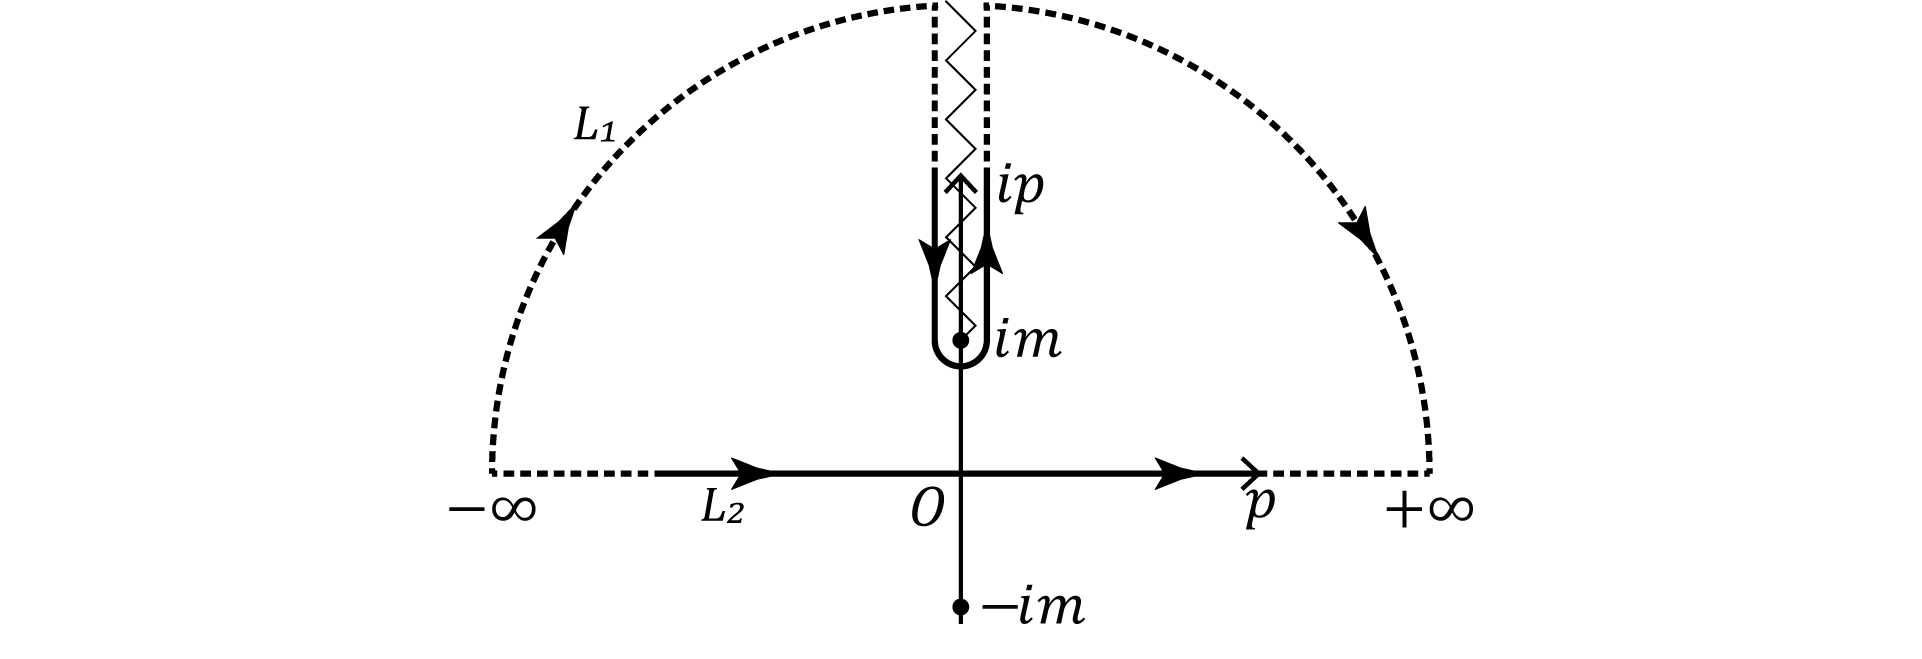
\includegraphics[width = 0.8\textwidth]{P27_2.52.png}
  \caption{push contour}
  \label{fig: pushcon}
\end{figure}

因此, 若记
\begin{equation}
  f(p) = \frac{pe^{ipr}}{\sqrt{p^2+m^2}}, 
\end{equation}
并将$p$视为复数, 则有
\begin{equation}\label{eq: push_contour}
  \begin{aligned}
    \int_{L_2}dp\ f(p) &= \int_{L_1}dp\ fp \\
    &= \int_{\gamma_2}p\ f(p) + \int_{\gamma_1}dp\ f(p), 
  \end{aligned}
\end{equation}
其中积分路径为
\begin{equation*}
  \begin{aligned}
    \gamma_1: p(\rho) = i\rho, \rho\in[m,+\infty], \\
    \gamma_2: p(\rho) = i\rho, \rho\in[+\infty,m],  
  \end{aligned}
\end{equation*}
这里选择从上半平面积分是因为当$|p|\to\infty$时, $f(p)$在上半平面一致收敛为0. 因此, 两个无穷大$1/4$圆弧上积分值为0; 再考虑到$im$处无穷小半圆弧上的积分值为0, 我们就得到了笔记 (\ref{eq: push_contour}) 式的第二行. 

点$p = \pm im$是$\sqrt{p^2+m^2}$的支点(branch point). 从分支左侧到右侧时, 需要考虑图 \ref{fig: pushcon} 中所示的分支切割(branch cut), 此时$p^2+m^2$获得了$2\pi$的相位, 即$\sqrt{p^2+m^2}$获得了相位$e^{i\pi}$. 因此, 
\begin{equation}
  \begin{aligned}
    \int_{L_2}dp\,f(p) &= \int_{\gamma_2}dp\,f(p) + \int_{\gamma_1}dp\,f(p)\\
    &= \int_{\gamma_2}dp\,\frac{pe^{ipr}}{\sqrt{p^2+m^2}}
    + \int_{\gamma_1}dp\,\frac{pe^{ipr}}{e^{i\pi}\sqrt{p^2+m^2}}\\
    &= -2\int_{\gamma_1}dp\,\frac{pe^{ipr}}{\sqrt{p^2+m^2}}\\
    &= 2i\int_{m}^{\infty}d\rho\,\frac{\rho e^{-\rho r}}{\sqrt{\rho^2-m^2}}, 
  \end{aligned}
\end{equation}
将积分结果带回即可得到书中(2.52)式. 

\subsubsection{P28 - (2.53)}

这个commutator用此笔记的 \ref{subsubsec: Invar_Delta} 中的$\Delta$可以表示为: 
\begin{equation}
  [\phi(x), \phi(y)] = i\Delta(x-y; m). 
\end{equation}

\begin{remark}
  可以这样解释的原因是: 在量子力学中我们将两个态的内积的模的平方解释为该态可被观测到的概率, 是可观测量. 而书中前面虽将$\phi(x) |0\rangle$类比为了$|x\rangle$, 但没有赋予其其他含义. (可以理解为这个传播振幅无法与可观测量联系起来, 故无法传递信息). 而算符$\phi(x), \phi(y)$的对易关系与量子力学中算符的对易关系的含义相同. 
\end{remark}

\subsubsection{P30 - (2.54)}

第二行第二项的$e$指数项中除了把$E_\mathbf{p}$写为了$-(-E_\mathbf{p})$以外, 还做了变换$\mathbf{p} \rightarrow -\mathbf{p}$. 

最后一步反着算比较容易: 在最后一行的式子中计算关于$p^0$的积分, 从下方闭合积分路径, 使用留数定理就可以得到第二行的表达式(最后一行表达式中的那个$(-1)$是因为从下方闭合了积分路径); 而这里当$(x_0 - y_0)>0$才从下方闭合积分路径的原因是只有这样$e^{-ip(x - y)}$才在无穷远处为零. 

\subsubsection{P30 - (2.56)}

首先注意: 
\begin{equation}
  \partial_\mu \theta(x^0) = g_{0\mu} \delta(x^0) \label{eq: partial_on_delta}.
\end{equation}

第一行: 对阶跃函数求一次导, 再应用分部积分后会得到
\begin{equation}
  \partial_0 \Bigl(\delta(x_0 - y_0)\langle 0|[\phi(x), \phi(y)]|0\rangle \Bigr)-\delta(x_0 - y_0)\partial_0\langle 0|[\phi(x), \phi(y)]|0\rangle,
\end{equation}
其中第一项等于0的原因可以粗略理解为: $x_0 \neq y_0$时, $\delta(x_0 - y_0)$等于0; $x_0 = y_0$时, $\langle 0|[\phi(x), \phi(y)]|0\rangle$等于0. 

第二行: 注意使用此笔记的 (\ref{eq: partial_on_delta}) 式及书中的(2.47). 

第三行: Klein-Gordon equation. 

\subsubsection{P30 - (2.57)}

给等式两边作用微分算符$(\partial^2 + m^2)$, 再比较两边的形式, 就可以得到(2.57)下面的表达式. 

\subsubsection{P31 - (2.59)}

这里极点的计算有个小trick: 我们得到$p^0 = \pm\sqrt{E_\mathbf{p}^2 - i\epsilon}$后, 对小量$\epsilon$展开可得$p^0 = \pm (E_\mathbf{p} - \frac{1}{2}i\epsilon)$, 这时只要令$\epsilon^* = \frac{1}{2}\epsilon$即可(都是同阶无穷小). 

\clearpage

\section{The Dirac Field}

\subsection{Lorentz Invariance in Wave Equations}

\begin{note}
  本书中的变换都是对场本身进行操作. (\textit{active} point of view)
\end{note}

\subsubsection{P36 - (3.3)}

这里只要把$(\Lambda^{-1}x)$看作是$x$的某个函数$y(x) = \Lambda^{-1}x$, 做复合函数的求导即可. 等式右端最后那个括号的意思是前面的函数$\partial_{\nu}\phi$在$\Lambda^{-1}x$处取值. 

\subsubsection{P39 - (3.15) (3.16)}

$J^3 = J^{12}$中, 3是(3.15)中的的上标, 12是中间没有序号的式子中的上标. 

从这里开始会用全反对称的张量来表示矢量. 它们所带有的信息是一样的, 只是形式上对称的量会更方便使用. 而同时, 后面的参数也被全反对称化了, 也因此多了个$1/2$的系数. 

\begin{remark}
  一开始学到这里的时候我很迷惑, 不过习惯了就好了. 对这些含有张量的表达式或运算感到疑惑的时候, 把分量具体写出来算一遍总是个好办法. 
\end{remark}

\subsubsection{P39 - (3.17)}

这是Lorentz Algebra的定义, 并不是由计算(3.16)的对易\textit{推导}出来的. 

\subsubsection{P39 - (3.18)}

洛伦兹群在矢量空间的具体表示. $\mu\nu$指标代表着6个洛伦兹变换(3个boost和3个rotation), $\alpha$和$\beta$代表矢量的4个分量. 

相当重要的一个例子, 后面也要用到. 
\begin{remark}
  注意区分矢量空间和其他表示空间 (基本都是旋量空间) 的指标. 一般后者会被省略. 
\end{remark}

\subsubsection{P40 - (3.19)}

写成有限形式就是$V' = \exp{(-\frac{i}{2}\omega_{\mu\nu}\mathcal{J}^{\mu\nu})}V$. (对比(3.13))

\subsection{The Dirac Equation}

\begin{note}
  狄拉克旋量具体可写为:  
  \begin{equation}
    \psi = \left( \begin{array}{c} \psi_1 \\ \psi_2 \\ \psi_3 \\ \psi_4 \end{array} \right), 
  \end{equation}
  其狄拉克共轭为: 
  \begin{equation}
    \overline{\psi} = \psi^\dagger \gamma^0 = (\psi^\dagger_1, \psi^\dagger_2, \psi^\dagger_3, \psi^\dagger_4)\gamma^0. 
  \end{equation}
\end{note}

\subsubsection{P40 - (3.23)}

\begin{equation}
  \begin{aligned}
    \relax
    [S^{\mu\nu}, S^{\rho\sigma}] &= \biggl[\frac{i}{4}(\gamma^\mu \gamma^\nu - \gamma^\nu \gamma^\mu), \ \frac{i}{4}(\gamma^\rho \gamma^\sigma - \gamma^\sigma \gamma^\rho)\biggr]\\
    &= \biggl(\frac{i}{4}\biggr)^2 \Bigl\{\gamma^\mu \gamma^\nu \gamma^\rho \gamma^\sigma - \gamma^\mu \gamma^\nu \gamma^\sigma \gamma^\rho - \gamma^\nu \gamma^\mu \gamma^\rho \gamma^\sigma + \gamma^\nu \gamma^\mu \gamma^\sigma \gamma^\rho \\ 
    &\qquad \quad \ \ - \gamma^\rho \gamma^\sigma \gamma^\mu \gamma^\nu + \gamma^\rho \gamma^\sigma \gamma^\nu \gamma^\mu + \gamma^\sigma \gamma^\rho \gamma^\mu \gamma^\nu - \gamma^\sigma \gamma^\rho \gamma^\nu \gamma^\mu \Bigr\}. 
  \end{aligned}
\end{equation}

注意到下面一行中上标的顺序恰好与上面一行的相反. 以第一项和最后一项为例子, 反复使用对易关系(3.22), 我们可以得到: 
\begin{equation}
  \begin{aligned}
    &\gamma^\mu \gamma^\nu \gamma^\rho \gamma^\sigma - \gamma^\sigma \gamma^\rho \gamma^\nu \gamma^\mu \\
    = &- 2g^{\mu\nu}\gamma^\sigma \gamma^\rho + 2g^{\mu\rho}\gamma^\sigma \gamma^\nu - 2g^{\mu\sigma}\gamma^\rho \gamma^\nu + 2g^{\nu\rho}\gamma^\mu \gamma^\sigma - 2g^{\nu\sigma}\gamma^\mu \gamma^\rho + 2g^{\rho\sigma}\gamma^\mu \gamma^\nu. 
  \end{aligned}
\end{equation}
计算其余三项时调整上标即可(善用文本编辑器的\textit{查找和替换}功能). 

大括号内结果: 
\begin{equation}
  \begin{aligned}
    &- 2g^{\mu\nu}\gamma^\sigma \gamma^\rho + 2g^{\mu\rho}\gamma^\sigma \gamma^\nu - 2g^{\mu\sigma}\gamma^\rho \gamma^\nu + 2g^{\nu\rho}\gamma^\mu \gamma^\sigma - 2g^{\nu\sigma}\gamma^\mu \gamma^\rho + 2g^{\rho\sigma}\gamma^\mu \gamma^\nu \\
    &+ 2g^{\mu\nu}\gamma^\rho \gamma^\sigma - 2g^{\mu\sigma}\gamma^\rho \gamma^\nu + 2g^{\mu\rho}\gamma^\sigma \gamma^\nu - 2g^{\nu\sigma}\gamma^\mu \gamma^\rho + 2g^{\nu\rho}\gamma^\mu \gamma^\sigma - 2g^{\sigma\rho}\gamma^\mu \gamma^\nu \\
    &+ 2g^{\nu\mu}\gamma^\sigma \gamma^\rho - 2g^{\nu\rho}\gamma^\sigma \gamma^\mu + 2g^{\nu\sigma}\gamma^\rho \gamma^\mu - 2g^{\mu\rho}\gamma^\nu \gamma^\sigma + 2g^{\mu\sigma}\gamma^\nu \gamma^\rho - 2g^{\rho\sigma}\gamma^\nu \gamma^\mu \\
    &- 2g^{\nu\mu}\gamma^\rho \gamma^\sigma + 2g^{\nu\sigma}\gamma^\rho \gamma^\mu - 2g^{\nu\rho}\gamma^\sigma \gamma^\mu + 2g^{\mu\sigma}\gamma^\nu \gamma^\rho - 2g^{\mu\rho}\gamma^\nu \gamma^\sigma + 2g^{\sigma\rho}\gamma^\nu \gamma^\mu,  
  \end{aligned}
\end{equation}
消项合并后可以得到: 
\begin{equation}
  -4g^{\mu\rho}[\gamma^\nu, \gamma^\sigma] + 4g^{\mu\sigma}[\gamma^\nu, \gamma^\rho] + 4g^{\nu\rho}[\gamma^\mu, \gamma^\sigma] - 4g^{\nu\sigma}[\gamma^\mu, \gamma^\rho],  
\end{equation}
考虑系数$(\frac{i}{4})^2$, 即可证明(3.23)满足(3.17).

\subsubsection{P42 - (3.28)下面的两个式子}

第一个式子的证明: 
\begin{equation}
  \begin{aligned}
    l.h.s &= \frac{i}{4}\bigl[\gamma^\mu, [\gamma^\rho, \gamma^\sigma]\bigr] \\
    &= \frac{i}{4}[\gamma^\mu, \gamma^\rho \gamma^\sigma] - \frac{i}{4}[\gamma^\mu, \gamma^\sigma \gamma^\rho] \\ 
    &= \frac{i}{4}\Bigl(\{\gamma^\mu, \gamma^\rho\}\gamma^\sigma - \gamma^\rho\{\gamma^\mu, \gamma^\sigma\} - \{\gamma^\mu, \gamma^\sigma\}\gamma^\rho + \gamma^\sigma\{\gamma^\mu, \gamma^\rho\}\Bigr) \\
    &= \frac{i}{4}\Bigl(2g^{\mu\rho}\gamma^\sigma - 2g^{\mu\sigma}\gamma^\rho - 2g^{\mu\sigma}\gamma^\rho + 2g^{\mu\rho}\gamma^\sigma \Bigr) \\
    &= i(g^{\mu\rho}\gamma^\sigma - g^{\mu\sigma}\gamma^\rho), \\
    \ \\
    r.h.s &= g^{\mu\lambda}(\mathcal{J}^{\rho\sigma})_{\lambda\nu} \gamma^\nu \\
    &= g^{\mu\lambda}\cdot i(\delta^\rho_{\phantom{1}\lambda} \delta^\sigma_{\phantom{1}\nu} - \delta^\rho_{\phantom{1}\nu} \delta^\sigma_{\phantom{1}\lambda}) \gamma^\nu \\ 
    &= i(g^{\mu\rho}\gamma^\sigma - g^{\mu\sigma}\gamma^\rho), 
  \end{aligned}
\end{equation}
$l.h.s = r.h.s$, 即证. 

第二个式子中, 把左边展开后忽略二阶小量即可. 

\subsubsection{P42 - (3.31)下方验证洛伦兹协变的式子}

对第一行的$\gamma^\mu \partial_\mu$做变换后会多出来一个$\Lambda^{-1}$的原因参考书中式(3.3).

\subsubsection{P43 - (3.35)}

小技巧: 
\begin{equation}
  \frac{\partial (\partial_\mu \phi)}{\partial (\partial_\nu \phi)} = \delta_\mu^{\phantom{1}\nu}, 
\end{equation}
相似地, 
\begin{equation}
  \frac{\partial (\partial_\mu A_\nu)}{\partial (\partial_\rho A_\sigma)} = \delta_\mu^{\phantom{1}\rho}\delta_\nu^{\phantom{1}\sigma}.
\end{equation}

\subsubsection{P44 - (3.38)}

注意这里的$\sigma^2$指$\sigma^i, i=2$. (我第一次遇见的时候以为是$\boldsymbol{\sigma}^2$, 想了老半天)

\subsection{Free-Particle Solutions of the Dirac Equation}

\subsubsection{P46 - (3.49)}\label{subsubsec: Boost_u_p}

\begin{enumerate}
  \item 最后一步要用到(3.48)的结果, 即$\sqrt{m}\ e^{\eta/2} = \sqrt{E + p^3}$, 以及$\sqrt{m}\ e^{-\eta/2} = \sqrt{E - p^3}$. 
  \item 若只考虑3-direction, 最终结果可以写为
  \begin{equation}
    \left( \begin{array}{c} \left( \begin{array}{cc} \sqrt{E-p^3} & 0 \\ 0 & \sqrt{E+p^3} \end{array} \right)\xi \\ \left( \begin{array}{cc} \sqrt{E+p^3} & 0 \\ 0 & \sqrt{E-p^3} \end{array} \right)\xi \end{array} \right), 
  \end{equation}
  \item 这里对$u(p_0)$进行boost后得到了$u(p)$, 完整形式实际上是$u'(\Lambda p_0) = \Lambda_{\frac{1}{2}}u(p_0)$ (boost后应有prime), 即$u'(p) = \Lambda_{\frac{1}{2}}u(\Lambda^{-1}p)$, 与书中(3.8)式形式一致. (在推导(3.110)时会用到)
  \begin{note}
    (3.8)是坐标空间下的变换规则, 但按照书中(3.2)式的思想, 动量空间中的变换规则也应该是一致的. 最直接的验证方法是将书中(3.46)式($u(p)$为满足此方程的解)写为$(\gamma^\mu(\Lambda p)_\mu - m)u(\Lambda p) = 0$, 利用书中(3.29)式得到含有$\Lambda_{1/2}$的形式后, 再和原式做比较. 

    \mbox{}

    附: 另外一个直接推导

    由于$\psi(x) = u(p)e^{-ip\cdot x}$, 所以进行变换$\psi(x) \rightarrow \psi'(x) = \Lambda_{\frac{1}{2}}\psi(\Lambda^{-1}x)$后, 对$u(p)$有
    \begin{equation}
      \begin{aligned}
        u'(p)e^{-ip\cdot x} &= \Lambda_{\frac{1}{2}}u(p)e^{-ip\cdot \Lambda^{-1}x} \\
        u'(p)e^{-ip\cdot x} &= \Lambda_{\frac{1}{2}}u(\Lambda^{-1}p')e^{-i\Lambda^{-1}p'\cdot \Lambda^{-1}x} \\
        u'(p)e^{-ip\cdot x} &= \Lambda_{\frac{1}{2}}u(\Lambda^{-1}p')e^{-ip'\cdot x}, 
      \end{aligned}
    \end{equation}
    所以对$\psi(x)$的做的变换实际上使得
    \begin{equation}
      u(p) \rightarrow u'(p) = \Lambda_{\frac{1}{2}}u(\Lambda^{-1}p). 
    \end{equation}
  \end{note}
\end{enumerate}

\subsubsection{P46 - (3.50)}

在只考虑3-direction时, $p\cdot \sigma = p^0 + p^3\sigma^3$, 已经是对角化的形式, 取正根即可. 

若考虑更一般的形式, 对(3.49)式的结果做替换$\sigma^3 \rightarrow \boldsymbol{\sigma}\cdot\hat{n},\ p^3 \rightarrow \mathbf{p}\cdot\hat{n}$, 其中$\hat{n} = \hat{p}$. 考虑第一个分量的平方
\begin{equation}
  \begin{aligned}
    &\biggl(\sqrt{E+\mathbf{p}\cdot\hat{n}} \frac{1-\boldsymbol{\sigma}\cdot\hat{n}}{2} + \sqrt{E-\mathbf{p}\cdot\hat{n}} \frac{1+\boldsymbol{\sigma}\cdot\hat{n}}{2} \biggr)^2 \\ 
    =& (E+\mathbf{p}\cdot\hat{n}) \frac{1-\boldsymbol{\sigma}\cdot\hat{n}}{2} + (E-\mathbf{p}\cdot\hat{n}) \frac{1+\boldsymbol{\sigma}\cdot\hat{n}}{2} + \sqrt{E^2 - (\mathbf{p}\cdot\hat{n})^2} \cdot 0 \\
    =& E - (\mathbf{p}\cdot\hat{n})(\boldsymbol{\sigma}\cdot\hat{n}) \\
    =& E - \mathbf{p} \cdot \boldsymbol{\sigma} \\
    =& p \cdot \sigma .
  \end{aligned}
\end{equation}

\subsubsection{P46 - (3.51)}

记得把(3.50)代回到(3.45)后再做计算. 

\subsection{Dirac Matrices and Dirac Field Bilinears}

\subsubsection{P50 - (3.72)}

这里可以自己验证一下$\bar{\psi} \gamma^5 \psi$在连续洛伦兹变换下是标量.

\subsubsection{P51 - (3.76)}

利用书中(3.72), 
\begin{equation}
  \biggl( \frac{1 - \gamma^5}{2} \biggr) \psi = \left( \begin{array}{cc} 1 & 0 \\ 0 & 0 \end{array} \right) \left( \begin{array}{c} \psi_L \\ \psi_R \end{array} \right) = \left( \begin{array}{c} \psi_L \\ 0 \end{array} \right), 
\end{equation}
而$\psi^\dagger \gamma^0 \gamma^\mu$中的两个$\gamma$相乘会得到对角形式的矩阵. 因此整个表达式只与$\psi_L$有关, 为左手流. 

\subsubsection{P51 - (3.77)}

建议对16个分量直接进行验证. 

\subsubsection{P51 - (3.78)}

将矩阵的元素(即带有下标的形式, 例如$\epsilon_{\alpha \gamma}$)具体写出来后, 由于这些元素只是数字(\textit{c-number}), 所以可以随便挪动位置. (矩阵乘法的分量形式: $(AB)_{ab} = \sum_c A_{ac} B_{cb}$) 后面的计算中经常要用到这个技巧. 

恒等式的证明: 
\begin{equation}
  \begin{aligned}
    l.h.s. &= (\bar{u}_{1R})_\alpha (u_{2R})_\beta (\bar{u}_{3R})_\gamma (u_{4R})_\delta (\sigma^{\mu})_{\alpha\beta} (\sigma_{\mu})_{\gamma\delta} \\
    &= (\bar{u}_{1R})_\alpha (u_{2R})_\beta (\bar{u}_{3R})_\gamma (u_{4R})_\delta (2\epsilon_{\alpha\gamma} \epsilon_{\beta\delta}) \\
    &= (\bar{u}_{1R})_\alpha (u_{2R})_\beta (\bar{u}_{3R})_\gamma (u_{4R})_\delta (-2\epsilon_{\alpha\gamma} \epsilon_{\delta\beta}) \\
    &= (\bar{u}_{1R})_\alpha (u_{2R})_\beta (\bar{u}_{3R})_\gamma (u_{4R})_\delta (\sigma^{\mu})_{\alpha\delta} (\sigma_{\mu})_{\gamma\beta} (-1) \\
    &= -(\bar{u}_{1R} \sigma^{\mu} u_{4R})(\bar{u}_{3R} \sigma_{\mu} u_{2R}), 
  \end{aligned}
\end{equation}
第三行中调换了$\beta$和$\delta$的位置. 

\subsection{Quantization of the Dirac Field}

\subsubsection{{P52} - (3.84)}
\begin{equation}
  \begin{aligned}
    \mathcal{H} &= i {\psi}^\dagger \dot{\psi} - \mathcal{L} \\
    &= i {\psi}^\dagger \dot{\psi} - i \bar{\psi} \gamma^0 \dot{\psi} - i \bar{\psi} \gamma^i \partial_i \psi \\
    &= {\psi}^\dagger (-i \gamma^i \partial_i + m) \psi. 
  \end{aligned}
\end{equation}

\begin{remark}
  注意$\gamma^\mu \partial_\mu = \gamma^0 \partial_0 + \gamma^i \partial_i$. 不要习惯性地写成减号. 
\end{remark}

\subsubsection{P54 - (3.90)}

利用$u^s(\mathbf{p})e^{i\mathbf{p} \cdot \mathbf{x}}$是$h_D$的本征函数的性质简化书中(3.84), 之后的计算很简单. 

\subsubsection{P59 - (3.110)附近}
\begin{enumerate}
  \item 注意$p\cdot x = \Lambda p\cdot \Lambda x$(书中(3.4)式).
  \item (3.110)上面一行里的那个关系在此笔记的 \ref{subsubsec: Boost_u_p} 中已经证明过了. 
\end{enumerate}

\subsection{Discrete Symmetries of the Dirac Theory}

\subsubsection{P67 - 中间没有序号的式子} 

这里是说$\psi(-t, \mathbf{x})|0\rangle$应该是正频项的和$e^{-iHt}\psi(\mathbf{x})|0\rangle$, 但用时间反演算符计算得到的结果却是负频项的和$e^{iHt}[T\psi(\mathbf{x})T]|0\rangle$. 它们之间是矛盾的. 

\subsubsection{P68 - (3.134)}

$\xi(\uparrow)$和$\xi(\downarrow)$是$\boldsymbol{\sigma}\cdot\mathbf{\hat{n}}$的本征态. 参见\textit{Modern Quantum Mechanics - J.J.Sakurai}: \textbf{Problem 1.9}. 

\subsubsection{P68 - (3.136)}

这里可以把$\eta^s$写为$\xi^{-s}$的原因在(3.112)上面的那一大段话中有讲.

\subsubsection{P70 - (3.147)}

关于这里第三步中出现的负号, 仍需讨论. 

\clearpage

\section{Interacting Fields and Feynman Diagrams}

\subsection{Perturbation Theory --- Philosophy and Examples}

跳过. 

\subsection{Perturbation Expansion of Correlation Functions}

\subsubsection{P84 - (4.21)}

Figure 4.1所表示的实际上是关于$T\{H_I(t_1) H_I(t_2)\}$的积分, 所以为了便于理解, 可以给等式左边的被积函数也加上编时记号$T$. 

图中上半三角上的积分可表示为
\begin{equation}
  \int_{t_0}^{t} dt_2 \int_{t_0}^{t_2} dt_1 T\{H_I(t_1) H_I(t_2)\}, 
\end{equation}
然后互换$t_1$, $t_2$, 由于编时记号的存在, 被积函数不变. 由此, 上半三角和下半三角上的积分完全相等. 

\begin{remark}
  也可以这么考虑: 由于编时记号的存在, 被积函数关于直线$t_1 = t_2$对称. 
\end{remark}

\subsubsection{P86 - (4.25)}

我们当然可以直接把(4.25)带入(4.24)来验证它是正确的, 但也可以由如下方法得到这个解: 
\begin{enumerate}
  \item 首先, (4.17)必然满足(4.24), 但它不满足边界条件($U = 1$ for $t = t'$); 
  \item 若采用(4.17)的形式, $U(t', t') = U(t', t_0) = e^{iH_0(t'-t_0)}e^{-iH(t'-t_0)}$为一\textit{常数}; 
  \item 给(4.17)左乘$U(t', t_0)^{-1} = e^{iH(t'-t_0)}e^{-iH_0(t'-t_0)}$, 那么此表达式必然满足(4.24)(只是乘了一个常数), 也必然满足边界条件($U(t', t_0)U(t', t_0)^{-1} = 1$). 
\end{enumerate}
最后得到的表达式即(4.25). 

\subsubsection{P87 - (4.29)}

这里是用$e^{-iHT}$从右侧作用到了$\langle 0|$上. 

\subsubsection{P87 - (4.31)}

把前面的表达式里的$U$都拆开以后再加上编时记号, 就可以随意挪动位置消项, 最后可以得到这个结果. 

\subsection{Wick's Theorem}

最后的证明展开后按正规序排好, 再反复使用$[A, BC] = B[A, C] + [A, B]C$即可. 

这里只给出了Bosonic field的Wick's Theorem, 对于Fermionic field, 还要根据场的对换次数确定符号(4.7节会讲). 

\subsection{Feynman Diagrams}

\subsubsection{P95 - \textit{momentum-space Feynman rules}}

其中第4条具体为: $(2\pi)^4 \delta(\sum\limits_i p_i)$. 

\subsubsection{P96 - (4.49)}

$(2\pi)^4 \delta(0)$可以理解为$\int d^4x e^{ip\cdot 0}$, 即$\int d^4x$, 其值为全空间体积($2T\cdot V)$. 

\subsubsection{P96 - (4.51)下面的式子}

\textit{The $1/n_i !$ is the symmetry factor coming from interchanging the $n_i$ copies of $V_i$.}
\begin{remark}[个人理解]\mbox{}
  
  这个对称系数来自于重复计算了“交换顶点”带来的系数, 即(4.45)下方的第一项所计算的\textit{interchange of vertices}. 

  对于由$x-y$和两个\textbf{8}字形的泡泡组成的费曼图来说, 交换两个泡泡的顶点是对称操作, 直接由Wick's theorem计算时并不会引入$2!$ (3个泡泡就是$3!$); 而若直接根据\textit{momentum-space Feynman rules}写出表达式时, 我们默认引入了这个系数并抵消掉了泰勒展开的系数, 因此这里需要给$V_i$乘$1/n_i !$. 

  对于其他的泡泡, 只有交换部分顶点才是对称操作, 因此经过计算总会得到$1/n_i !$这个系数(可以试试算两个“糖葫芦形”的泡泡). 不过这也是合理的, 因为忽略内部的顶点交换的话, “交换顶点”在某种程度上和“交换两个图”是一样的. 因此最后效果就是书中所说的\textit{The $1/n_i !$ is the symmetry factor coming from interchanging the $n_i$ copies of $V_i$.}

\end{remark}

\subsubsection{P97 - (4.52)}

关于怎么由上面的式子得到本式的第一行: 注意这里的每一个$n_i$的取值范围都是0到$\infty$, 无论是先乘后加还是先加后乘, 展开后得到的结果都是一样的. 可以试着算一个具体的有限的例子, 譬如$i = 1, 2, 3$, $n_i = 0, 1$.   

\subsection{Cross Sections and the \textit{S}-Matrix}

这一节讲怎么由$S$-Matrix计算截面. 最重要的公式是书中的(4.79)和(4.86). 

\subsubsection{P100 - (4.59) \& P101 - (4.62)}

把这两个式子当作截面和衰变率的定义记下来就可以, QFT里的定义是最好的定义. 

\subsubsection{P102 - (4.65)}

用$\langle \mathbf{x}|$同时作用在等式两边: 
\begin{equation}
  \begin{aligned}
    l.h.s. &= \langle \mathbf{x}|\phi \rangle = \phi(\mathbf{x}) \\ 
    r.h.s. &= \int\frac{d^3 k}{(2\pi)^3}\frac{1}{\sqrt{2E_{\mathbf{k}}}}\phi(\mathbf{k})\langle \mathbf{x}|\mathbf{k} \rangle \\
    &= \int\frac{d^3 k}{(2\pi)^3}\frac{1}{\sqrt{2E_{\mathbf{k}}}}\phi(\mathbf{k})\sqrt{2E_{\mathbf{k}}}\langle \mathbf{x}|a^{\dagger}_{\mathbf{k}}|0 \rangle \\
    &= \int\frac{d^3 k}{(2\pi)^3}\ e^{i\mathbf{k}\cdot\mathbf{x}}\phi(\mathbf{k}) \\
    &= \phi(\mathbf{x}).
  \end{aligned}
\end{equation}

\subsubsection{P102最下面的一大段话}

\begin{remark}[个人理解]
  中间的“Note that we use the Heisenberg picture:...”这一段是在说in state和out state是由含时算符的本征态建立的, 而这些算符本身会随着时间演化, 因此它们不共用同一组基, 所以它们之间会有nontrivial overlap. 
\end{remark}

\subsubsection{P103 - (4.68)}

式中的$e^{-i\mathbf{b}\cdot\mathbf{k_{\mathcal{B}}}}$是\textbf{平移算符}(translation operator). 可以参考J. J. Sakurai书中(1.6.32)式附近的说明. 

\subsubsection{P104 - (4.74)}

因为考虑的是落在$d^3p_1\cdots d^3p_n$这个小区域里的概率, 所以这里的$\mathcal{P}$应该写为$d\mathcal{P}$. 也因此, 等式右侧只有一个积分号, 利用书中(4.66)式可以将所有$|\phi(\mathbf{p}_n)|^2$归一化得到分子上那个$1$. 

\subsubsection{P105 - (4.77)}

最后一行利用笔记中(\ref{eq: delta_on_function})式计算即可. 

关于$k_{\mathcal{A}}^{\bot}$: 

由
\begin{gather}
  \delta^{(4)}(\sum k_i - \sum p_f) \\
  \delta^{(4)}(\sum \bar{k}_i - \sum p_f)
\end{gather}
可以得到
\begin{equation}
  k_\mathcal{A} + k_\mathcal{B} = \bar{k}_\mathcal{A} + \bar{k}_\mathcal{B}, 
\end{equation}
只考虑$\bot$分量: 
\begin{equation}
  k_{\mathcal{A}}^{\bot} + k_{\mathcal{B}}^{\bot} = \bar{k}_{\mathcal{A}}^{\bot} + \bar{k}_{\mathcal{B}}^{\bot}, 
\end{equation}
再考虑$\delta^{(2)}(k_{\mathcal{B}}^{\bot} - \bar{k}_{\mathcal{B}}^{\bot})$, 则有
\begin{equation}
  k_{\mathcal{A}}^{\bot} = \bar{k}_{\mathcal{A}}^{\bot}, 
\end{equation}
即$\delta^{(2)}(k_{\mathcal{A}}^{\bot} - \bar{k}_{\mathcal{A}}^{\bot})$.

\subsubsection{P106 - (4.78)}

这里是把$\mathbf{k}_{\mathcal{A}}, \mathbf{k}_{\mathcal{B}}, \bar{\mathbf{k}}_{\mathcal{A}}, \bar{\mathbf{k}}_{\mathcal{B}}$全部用中心值$\mathbf{p}_{\mathcal{A}}, \mathbf{p}_{\mathcal{B}}$代替了. 

\subsection{Computing \textit{S}-Matrix Elements from Feynman Diagrams}

这一节最重要的是书中的(4.103)和(4.104)两式, 以及配套的Feynman rules. 

\subsubsection{P109 - (4.89)}

$e^{-iH(2t)}$可以写为$T(\exp[-i\int_{-T}^{T}dt\ H_I(t)])$的原因参考书中(4.28)和(4.29).

\subsection{Feynman Rules for Fermions}

\subsubsection{P119最上方的费曼图中的动量方向}

前面一段话里提到了初态粒子对应入射(ingoing)动量, 而由于这种态总是与$\psi$或$\bar{\psi}$中的$a_{\mathbf{p}}$或$b_{\mathbf{p}}$形成contraction, 并且会乘上$e^{-ip\cdot x}$, 故$e^{-ip\cdot x}$总是对应着入射(ingoing)动量. 反之, $e^{+ip\cdot x}$总是对应着出射(outgoing)动量. 

根据这个规则, 可以由书中费曼图底下式子中的$e^{-iq\cdot (x-y)}$一项确定费曼图中的动量方向. 

\subsection{Feynman Rules for Quantum Electrodynamics}

\clearpage

\section{Elementary Processes of Quantum Electrodynamics}

\subsection{\texorpdfstring{$e^+e^- \rightarrow \mu^+\mu^-$}:: Introduction}

\subsubsection{P132 - (5.2)上面那个式子}

由于$\mathcal{M}$只是个\textit{c-number}, 并非矩阵, 故$\mathcal{M}^\dagger = \mathcal{M}^*$

\subsubsection{P132 - (5.3)上面那个求平均}

考虑入射粒子流由$n$种不同的粒子组成, 发现每种粒子的概率为$p_n(\sum p_n = 1)$, 那么总截面即为每种粒子的分截面的总和, 即
\begin{equation}
  |\mathcal{M}|^2 = \sum p_n |\mathcal{M}_n|^2, 
\end{equation}
书中的例子考虑了自旋向上或向下的概率为$1/2$, 即完全非极化的情况. 

由于入射流的粒子情况是已知的, 粒子总数目固定, 每种粒子所占的比例已知, 所以求总截面时计算各分截面的期望; 而出射流的粒子情况未知, 探测器忽略了自旋信息, 故需对所有类型的事件的数目直接求和. 

\subsection{\texorpdfstring{$e^+e^- \rightarrow \mu^+\mu^-$}:: Helicity Structure}




\clearpage

\section{Radiative Corrections: Introduction}

\section{Radiative Corrections: Some Formal Developments}

\clearpage

\section{Invitation: Ultraviolet Cutoffs and Critical Fluctuations}

介绍性的章节. 

可能有一些有意思的内容, 暂时跳过. 

\clearpage

\section{Functional Methods}

\subsection{Path Integrals in Quantum Mechanics}

这一节随便看看就行了, 推荐去看Sakurai或者Srednicki相关的部分. 下一节开始才是重要的部分. 

\subsubsection{P276 - (9.2)}

参考书中(9.1), $U(x_a, x_b; T)$实际上有着$e^{i \cdot (\text{phase})}$的形式. 

\subsubsection{P278 - (9.4)}

\begin{remark}
  简单的理解: 把一条路径看成有无限个自变量($x_n, n \rightarrow \infty$)的多元函数, 那么在这个由$x_n$张成的希尔伯特空间里积分的形式即为本式等号右边的形式. 
\end{remark}

\subsubsection{P279 - (9.5)}

第一行的$[1-\frac{i\epsilon}{\hbar}V(x_b)+\cdots]$是展开两次后的结果: 先做近似$\exp(f(x)) = 1 + f(x) + \cdots$, 再对$V(\frac{x_b + x'}{2})$在$x_b$附近做泰勒展开.  

\subsubsection{P281 - Weyl order}

第一项中的$q$向左作用在bra上, 第二项中左右各一个, 第三项向右作用在ket上, 这种排序下左侧的结果和右侧的一致. 

\subsection{Functional Quantization of Scalar Fields}

\subsubsection{P282 - (9.14)}

\begin{remark}
  自己的理解: 考虑离散形式(9.11)的话, 利用高斯积分积掉$\pi$的相关项就很自然了(不用考虑指数上那个对时间$t$的积分). 
\end{remark}

\subsection{The Analogy Between Quantum Field Theory and Statistical Mechanics}



\clearpage

\section{Systematics of Renormalization}

\section{Renormalization and Symmetry}

\section{The Renormalization Group}

\section{Critical Exponents and Scalar Field Theory}

\clearpage

\section{Invitation: The Parton Model of Hadron Structure}

介绍性的章节. 

可能有一些有意思的内容, 暂时跳过. 

\clearpage

\section{Non-Abelian Gauge Invariance}

\subsection{The Geometry of Gauge Invariance}




% \section{Cheat Sheet}

% \subsection{定理类环境}

% \begin{theorem}[名称]
%   这是一个定理(theorem)
% \end{theorem}

% \begin{lemma}[名称]
%   这是一个引理(lemma)
% \end{lemma}

% \begin{proposition}[名称]
%   这是一个命题(proposition)
% \end{proposition}

% \begin{corollary}[名称]
%   这是一个推论(corollary)
% \end{corollary}

% \subsection{定义类环境}

% \begin{definition}[名称]
%   这是一个定义(definition)
% \end{definition}

% \begin{conjecture}[名称]
%   这是一个猜想(conjecture)
% \end{conjecture}

% \begin{example}[名称]
%   这是一个例子(example)
% \end{example}

% \subsection{备注类环境}

% \begin{remark}[名称]
%   这是一条评论(remark)
% \end{remark}

% \begin{note}[名称]
%   这是一条注(note)
% \end{note}

% \begin{case}[名称]
%   这是一个案例(case)
% \end{case}

% \subsection{证明类环境}

% \begin{proof}
%   这是一个证明(proof)
% \end{proof}

\end{document}


% 波浪线:\textasciitilde